% Use class option [extendedabs] to prepare the 1-page extended abstract.
\documentclass[extendedabs]{bmvc2k}
\usepackage[colorlinks = true,
            linkcolor = blue,
            urlcolor  = blue,
            citecolor = blue,
            anchorcolor = blue]{hyperref}
\usepackage{kotex} % 한국어 사용 가능

% Document starts here
\begin{document}
\title{GAN}
\addauthor{
Lee Gwan Hui$^1$, \today}{}{1}
\addinstitution{
$^1$2017142136, Department of Electrical and Electronic Engineering, Yonsei University.}
\maketitle
\let\thefootnote\relax\footnote{This is an extended abstract. The full paper is available at the \href{https://github.com/LeeGwanHui/TIL/tree/main/deeplearning_ham}{github}. }
\vspace{-0.2in}

\section{GAN\cite{goodfellow2014generative}}
 \subsection{motivation}
  \quad 기존의 deep learning model은 backpropagation과 dropout algorithm을 이용하여 큰 성공을 거두었는데 generative model의 경우에는 
  확률적 계산을 근사하는 어려움 때문에 골머리를 앓아왔다. 그래서 이 논문에서는 이 같은 어려움을 해결한 generative model을 제안한다.

 \subsection{model의 형태\cite{youtube_GAN}}
 \quad 이 논문에서 제시하는 GAN은 두가지 모델이 결합된 형태이다.
 \newline  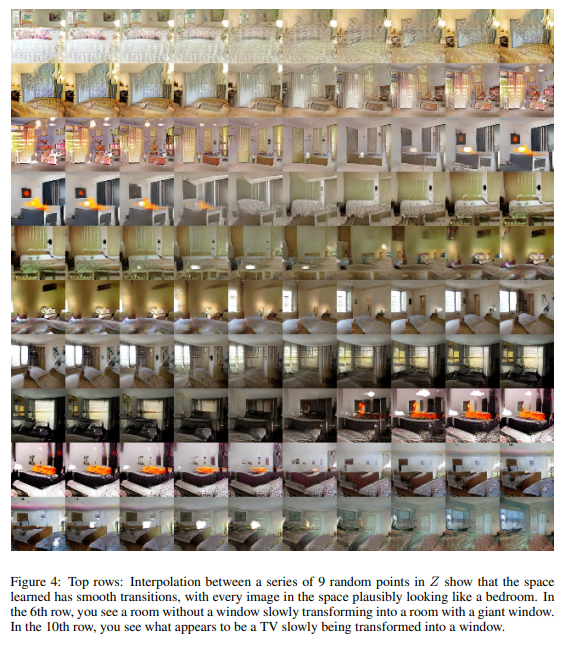
\includegraphics[width=6cm]{images/05_DCGAN.PNG}
 \newline GAN은 discriminative model과 generative model로 나눌 수 있다. discriminative model은 비유적으로 경찰에 해당하며 generative model이 만든 이미지가 
 fake 이미지인지를 판별하는 역할을 한다. 반면 위조지폐범으로 비유되는 generative model은 경찰에 안걸리도록 이미지를 real과 흡사하게 생성하게 된다.
 이를 수식으로 표현하면 아래와 같다. 
 $$ \underset{G}{min}\underset{D}{max}V(D,G) = E_{x ~ p_{data}(x)}[log D(x)] + E_{z~p_z(z)}[log(1-D(G(z)))] $$
 위의 식의 의미가 GAN에서는 매우 중요한데 D와 G의 model이 각각 다른 방향성으로 학습된다는 것이 중요하다. 
 D의 경우에는 generator가 만든 이미지가 잘못되었다는 것을 판단해야 하므로 최대가 되도록 학습되어야 한다. D(x)의 정확한 의미는 x가 생성된 이미지의 분포 $p_g$가 아닌 
 dataset에서 온 확률을 의미하는 것으로 fake가 들어오면 0을 real이 들어오면 1을 학습시켜야 한다. G는 반면 training data 분포와의 차이가 최소화 되도록 학습되어야 한다.
 이를 그림으로 표현하면 아래와 같다.
 \newline  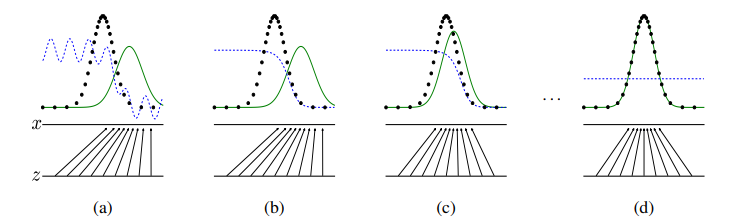
\includegraphics[width=\linewidth]{images/06_GAN.PNG}
 위의 그림은 실제 구조와는 차이가 있는 그림 설명이지만 학습과정을 이해하기에는 무리가 없다. 
 위의 그림에서 D가 의미하는 것은 파란색 선이고 training data는 검은색 generative data의 분포는 초록색으로 나타낸다. 
 학습과정에서 초록색 선은 검은색에 일치하도록 학습이 되어 D가 판별하는 확률이 1/2로 판별을 못할때가 optimal solution이 된다.
 즉 과정의 흐름을 살펴보자면 초기 학습이 진행되지 않은 상태가 (a)의 그림이다. 그리고 (b)는 D가 학습된 것으로 파란색이 real 부분에서는 1로
 generator가 만든 분포에 대해서는 0으로 되도록 함수가 그려진다. 이 D를 바탕으로 다시 G가 학습되어 training dataset의 분포와의 차이를 줄인 그림이 (c)이다.
 이과정을 반복하면 optimal solution인 (d)을 얻을 수 있는 것이다. 여기서 D와 G을 번갈아 가면서 학습하는 것은 아직 확실하지 않은 생성 그림에 과적합되지 않도록 하기 위해서 이다.
 초창기에는 log(1-D(G(z)))을 최소화하기 보다는 logD(G(z))을 최대화하는 방법을 사용해서 학습 속도를 올리기도 한다.
 이 논문에서는 이 model의 형태가 이론적으로 왜 적절한 이미지를 추출할 수 있는지를 증명하는 것을 중요하게 판단한다. 
 그 전에 알고리즘을 설명하자면 D(k step)와 G가 번갈이 가며 학습되며 각기 gradient을 ascending과 descending 함으로써 학습 방향이 다르다.
 왜  Global Optimality of $p_g = p_{data}$ 인지를 알아보자. 그 이유는 
 $$ V(D,G) = E_{x ~ p_{data}(x)}[log D(x)] + E_{z~p_z(z)}[log(1-D(G(z)))] = $$
 $$ = \int_{x} p_{data}(x)log(D(x)) dx + \int_{z} p_z(z)log(1-D(g(z)))dz$$
 $$ = \int_{x} p_{data}(x)log(D(x)) + p_g(x)log(1-D(x)) dx $$
 위의 식을 통해서 증명할 수 있다. 이 식을 이용하기 위해서는 y -> alog(y) + b log(1-y)를 maximum은 $\frac{a}{a+b}$ 이라는 것을 알아야한다. 
 이 답이 나오는 이유는 미분해서 0이 되는 y값을 찾으면 알 수 있다. 그래서 G가 고정되어 있을 때 D의 optimal discriminator 값이 아래와 같다.
 $$D_G^*(x) = \frac{p_{data}(x)}{p_{data}(x)+p_g(x)}$$
 이제 이를 바탕으로 왜 global optimum point가 $p_g = p_{data}$ 인지를 알아보자. 이 자료는 위의 model 형태의 출처에 있는 자료를 가져왔다.
 \newline  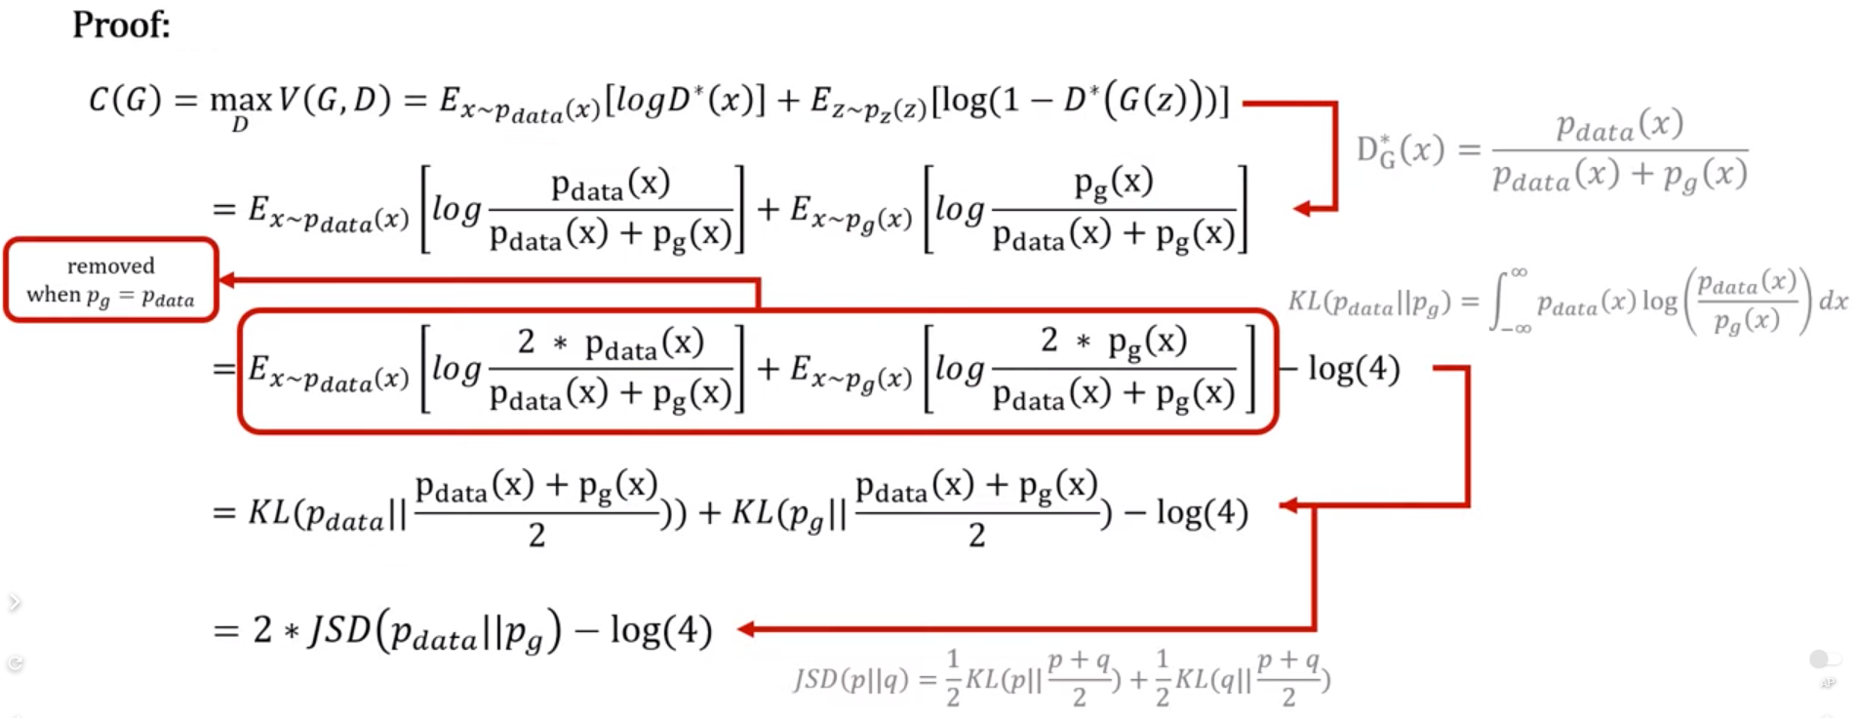
\includegraphics[width=\linewidth]{images/07_GAN.PNG}
 위의 식에서 JSD는 두개의 분포의 차이를 나타낸다. 즉 0이상의 값으로써 최솟값이 $p_g = p_{data}$인 상태에서 0이 되는데 이 때 C(G)의 값이 -log4의 값을 가지게 된다. 
 여기서 말하는 C(G)는 global minimum of the virtual training criterion 을 의미한다. 위의 식을 구지 변형시키는 이유는 JSD로 표현하기 위해서이다.

 \subsection{Experiments}
 \quad 이 모델을 MNIST, Toronto Face Database (TFD) , and CIFAR-10 dataset을 사용해서 검증했다. 
 generator의 경우에는 ReLU와 sigmoid activation이 사용되었다. 반면 discriminator의 경우에는 maxout activation을 사용하였다.
 Dropout은 discriminator에 적용하였다. 아래 자료는 GAN의 성능을 평가한 것이다. 다만 이 당시에는 
 Generator의 성능지표가 명확히 확립된 시기가 아니라서 저자가 실험시에 가장 적합하다고 생각한 성능지표를 사용했다고 한다.
 \newline  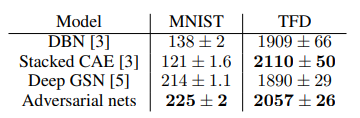
\includegraphics[width=6cm]{images/08_GAN.PNG}
 \newline 아래 그림은 생성된 모델로 맨 오른쪽의 그림은 training sample로 단순히 생성한 이미지가 복사된 결과가 아님을 보여준다.
 \newline  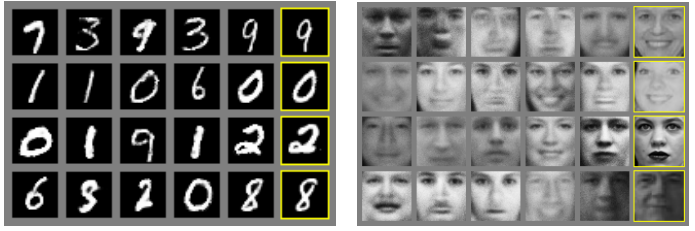
\includegraphics[width=\linewidth]{images/09_GAN.PNG}

 \subsection{Conclusion}
 \quad 결론을 보자면 Generator model을 두 개의 model인 discriminator과 generator을 사용해서 구현하였다. 이는 minmax game player과 같으며 이 때문에 
 적대적이라는 의미인 Adversarial 용어가 붙었다. 이 논문에서는 왜 GAN이 training dataeset의 특징을 추출하여 그와 비슷한 이미지를 생성해 내는지를 수학적으로 증명함으로써
 이 모델이 수렴할 수 있는 근거를 제시한다. 또한 이 GAN의 경우에는 backpropagation으로만 학습할 수 있기 때문에 기존의 generator model보다 더 편리한 모델이라고도 볼 수 있다.
 특징적으로 보자면 G와 D는 성능차이가 많이 나면 안된다. 많이 날 경우 학습속도가 매우 떨어진다는 단점이 있다.

 \section{DCGAN\cite{radford2015unsupervised}}
 \subsection{motivation}
 \quad CNN을 이용한 unsupervised learning은 supervised learning에 비해 집중을 덜 받았는데 이 논문에서는
 이 격차를 해소하는 DCGANs을 사용한 unsupervised learning을 다룰 것이다. 앞선 논문 GAN에서 이미지의 재사용이 가능한 feature을 가지고 
 학습을 진행하는 연구가 이루어졌는데 GAN은 이미지의 재표현 뿐만 아니라 generator과 discriminator을 적절히 이용해서 feature extractors로써도 
 사용가능하다. 하지만 결정적으로 loss를 업데이트 시키는 측면에서 한쪽은 -방향으로 다른쪽은 +방향으로 학습이 진행되는 unstable 단점이 있었다.
 또한 자주 generator에서 생성한 이미지가 적절하지 않다는 단점이 있다. 이 논문에서는 이러한 GAN의 단점을 보완하고자 최신 연구들을 응용하여 GAN의 구조를 
 변경한 새로운 model DCGANs을 제시한다.

 \subsection{model의 형태\cite{youtube}}
 \quad 이 논문에서는 주로 앞선 연구들을 종합시켜 좋은 성능을 낼 수 있는 모델을 만들었다는 특징이 있다. 크게 세가지의 접근법을 가졌다.
 첫째로는 pooling 방법으로 downsampling하는 것을 strided convolution으로 대체하는 것이다. 또한 upsampling 역시 transposed convolution을 사용할 것인데
 이는 upsampling, downsampling 하는 방법 조차 학습을 진행하여 더 높은 퀄리티의 이미지를 얻을 수 있다는 장점이 있다. 두번째로는 convolutional layer 뒤에 classifier로 추가되는 FC layer를 제거해주는 것이다.
 이 방법대신 Global average pooling을 사용할 것이다. 세번째는 batch normalization의 적용이다. 이는 convolutional layer을 통과하면서 데이터의 분포가 biased되는 것을 보정해주는 효과가 있어서 
 학습이 효율적으로 진행된다. DCGAN generator은 LSUN scene modeling을 사용했다. 그 구조는 아래와 같다.
 \newline  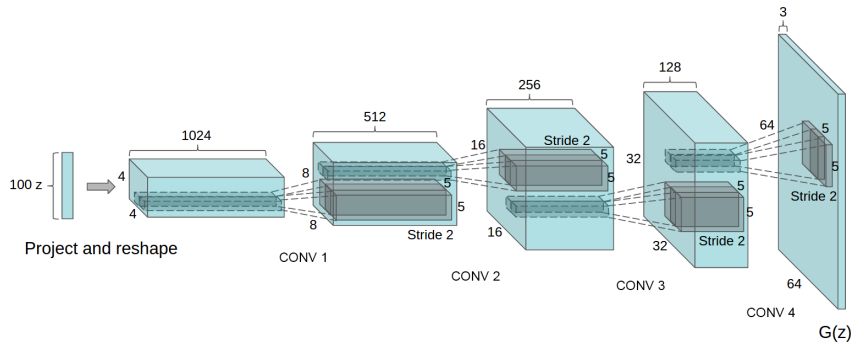
\includegraphics[width=\linewidth]{images/00_DCGAN.PNG}
 위의 그림에서 100z는 noise vector을 의미한다. 이게 입력으로 들어가서 convolutional network를 통과하여 64x64까지 증가시킬 수 있게 convolutional 연산으로 upsampling을 진행해준다.
 중간 중간 batch normalization도 적용해준다. ReLU activation을 사용하다가 마지막에서만 tanh를 사용한다. 

 \subsection{Experiments}
 \quad 이 실험에서는 크게 3가지 dataset에서 실험을 진행하였다. Large-Scale Scene Understanding(LSUN)으로 bedroom datset을 의미하고
 Imagenet-1k, Faces dataset에서도 진행하였다. training setting은 전처리를 training image에 하지 않았고 데이터 증강 기법도 사용하지 않았다. 또한 
 mini-batch SGD를 사용했고 이때 batch size는 128로 설정했다. weight은 standard deviation를 0.02로 설정한 zero-centered Normal distribution으로 초기화한다.
 그외에도 activation function은 LeakyReLU의 slope는 0.2로 두었다. 또한 Adam optimizer을 사용했다. learning rate는 0.001로 설정했다. 이렇게 아래와 같은 그림을 생성할 수 있었다.
 \newline  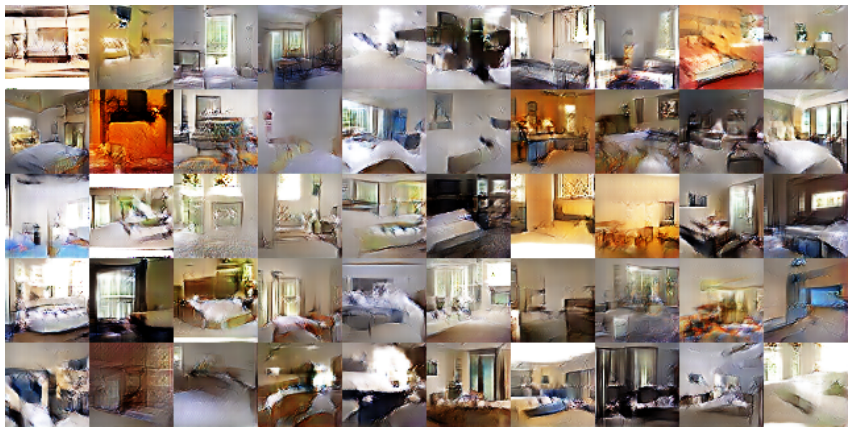
\includegraphics[width=6cm]{images/01_DCGAN.PNG}
 \newline 다양하게 DCGAN이 이미지를 어떤 방법으로 재표현하는 것인지에 대한 의문을 던지고 여러개의 실험을 진행한다. 먼저 feature extractor로써 GAN이 잘 작동하는지를 살펴보기 위해
 CUFAR-10 dataset을 기준으로 실험을 진행했다.
 \newline  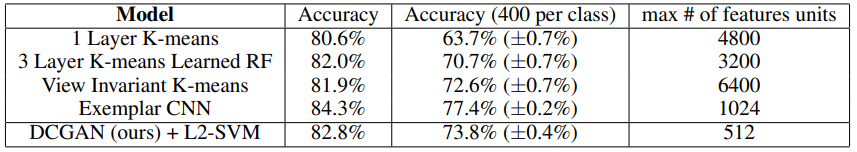
\includegraphics[width=\linewidth]{images/02_DCGAN.PNG}
 위의 결과는 discriminator에서 convolutional feature을 뽑아내고 L2-SVM을 사용해서 classification을 진행한 것이다. 성능이 classification에서도 괜찮다는 것을 볼 수 있다.
 다시 말해 물체의 feature을 추출한다는 의미이다. 또한 SYHN dataset에서도 진행해본 결과 CNN 구조만이 모델 성능의 key contributor factor이 아닌 것이라고 주장한다.
 그 근거로  같은 구조로 supervise CNN을 사용했을 때보다 성능이 좋았기 때문이라는 이유를 든다. 즉 CNN만이 아니라 GAN의 discriminator와 generator사이의 상호작용도 feature extractors의 동작을 작용해서 DCGAN의 성능이 좋다는 것이다.
 이 외에도 중간 CNN의 filter을 뽑아서 각 feature이 어떤 사물을 주목하고 있는지를 뽑아낸 실험, 이미지의 변화과정이 연속적임을 보여주는 실험도 있다.
 그 중에서 generator에서 window에 해당하는 feature을 bounding box를 이용해서 제거해보고 이미지를 생성했을 때 진짜 window가 없어지는지에 대한 실험도 진행하였는데 그 결과가 아래와 같다.
 \newline  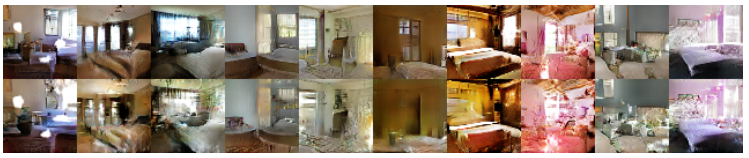
\includegraphics[width=\linewidth]{images/03_DCGAN.PNG}
 위의 결과를 보면 window가 다른 object로 대체되었음을 확인할 수 있다.
 또한 이미지를 vector arithmetic을 진행한 결과도 있는데 이는 예를 들면 이미지를 text화 해서 그 특징을 나열하고 그 특징 들간의 더하고 빼는 방식으로 새로운 이미지를 만들 수 있는지에 대한 실험이다.
 king이라는 vector에서 man을 빼고 woman이라는 vector을 더하면 queen에 가까운 이미지가 생성되는 것을 예로 들 수 있다. 결과는 아래와 같다.
 \newline  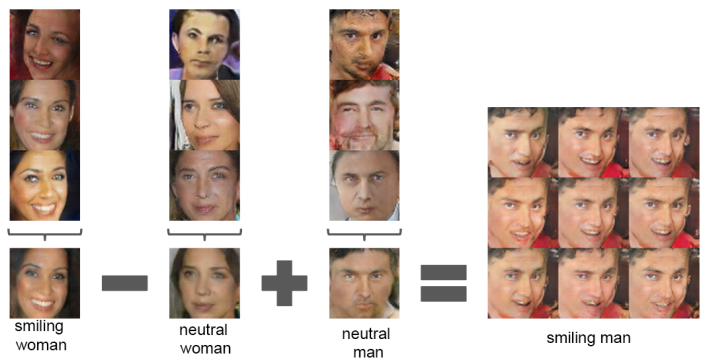
\includegraphics[width=6cm]{images/04_DCGAN.PNG}
 \newline 이 실험들을 통해서 알 수 있는 것은 DCGAN이 이미지를 복사해서 생성하는 것이 아니라 직접 특징들을 학습하고 그 특징을 바탕으로 적절한 이미지를 생성한다는 것이다.

 \subsection{Conclusion}
 \quad 이 논문에서는 보다 stable한 구조의 DCGANs을 제시하였다. 또한 제시한 모델 DCGAN이 이미지 representations을 할때 이미지의 feature을 바탕으로 의미있는 이미지를 
 생성해낸다는 것을 다양한 실험을 통해 증명하였다. 이 실험의 한계로써는 model이 train이 길어질 때 때때로 single oscillating mode에서
 filter간의 collapse가 일어나기 때문에 여전히 model이 instability하다는 점이다.
 그래서 앞으로의 연구는 instability을 해결하고 GAN의 활용을 video나 audio등으로 확장하는 것에 있다.

\newpage
\bibliography{egbib}

\end{document}